\chapter{Konzept}
\label{section:konzept}

Die Bachelorarbeit beschäftigt sich mit der Darstellung von Requirements in AR.
Dabei soll untersucht werden, wie Anforderungen in einer 3D-Umgebung dargestellt werden könnten.
Dazu werden verschiedene Interaktionskonzepte entwickelt, welche als Basis für die Implementierung von Prototypen mit WebXR dienen.
Die erste Ausarbeitung der Konzepte dient dabei nicht unbedingt dazu vollständig so implementiert zu werden, sondern soll einen Überblick über die grundlegende Idee und die möglichen Interaktionen geben.

\section{Explodierende Bauteile}

Das erste untersuchte Interaktionskonzept ist hauptsächlich für die Darstellung von Anforderungen von Produkten gedacht.
Die Idee ist, ein Produkt in einer Animation in seine einzelnen Bauteile zu zerlegen und die Anforderungen auf ihren zugehörigen Bauteilen darzustellen.
In der Animation werden die Bauteile wie in der Bildsequenz in Abbildung \ref{fig:rubiks-explosion} von einem Punkt in der Mitte des Produkts nach außen bewegt, sodass sie sich um den Ursprungspunkt des Produkts herum anordnen.
Beispielsweise könnte ein Auto so zerlegt werden, dass bei der Animation die Räder, die Karosserie, der Motor und die Innenausstattung einzeln als eigene Objekte sichtbar werden.
So kann der Nutzer das gesamte Produkt betrachten und sich dann auf Wunsch einzelne Bauteile und deren Anforderungen genauer ansehen.
Im Beispiel des Rubiks Cube aus Abbildung \ref{fig:rubiks-explosion} wäre dann jeder Würfel ein Bauteil, der seine eigenen Requirements angehängt bekommen würde.

\begin{figure}[H]
    \centering
    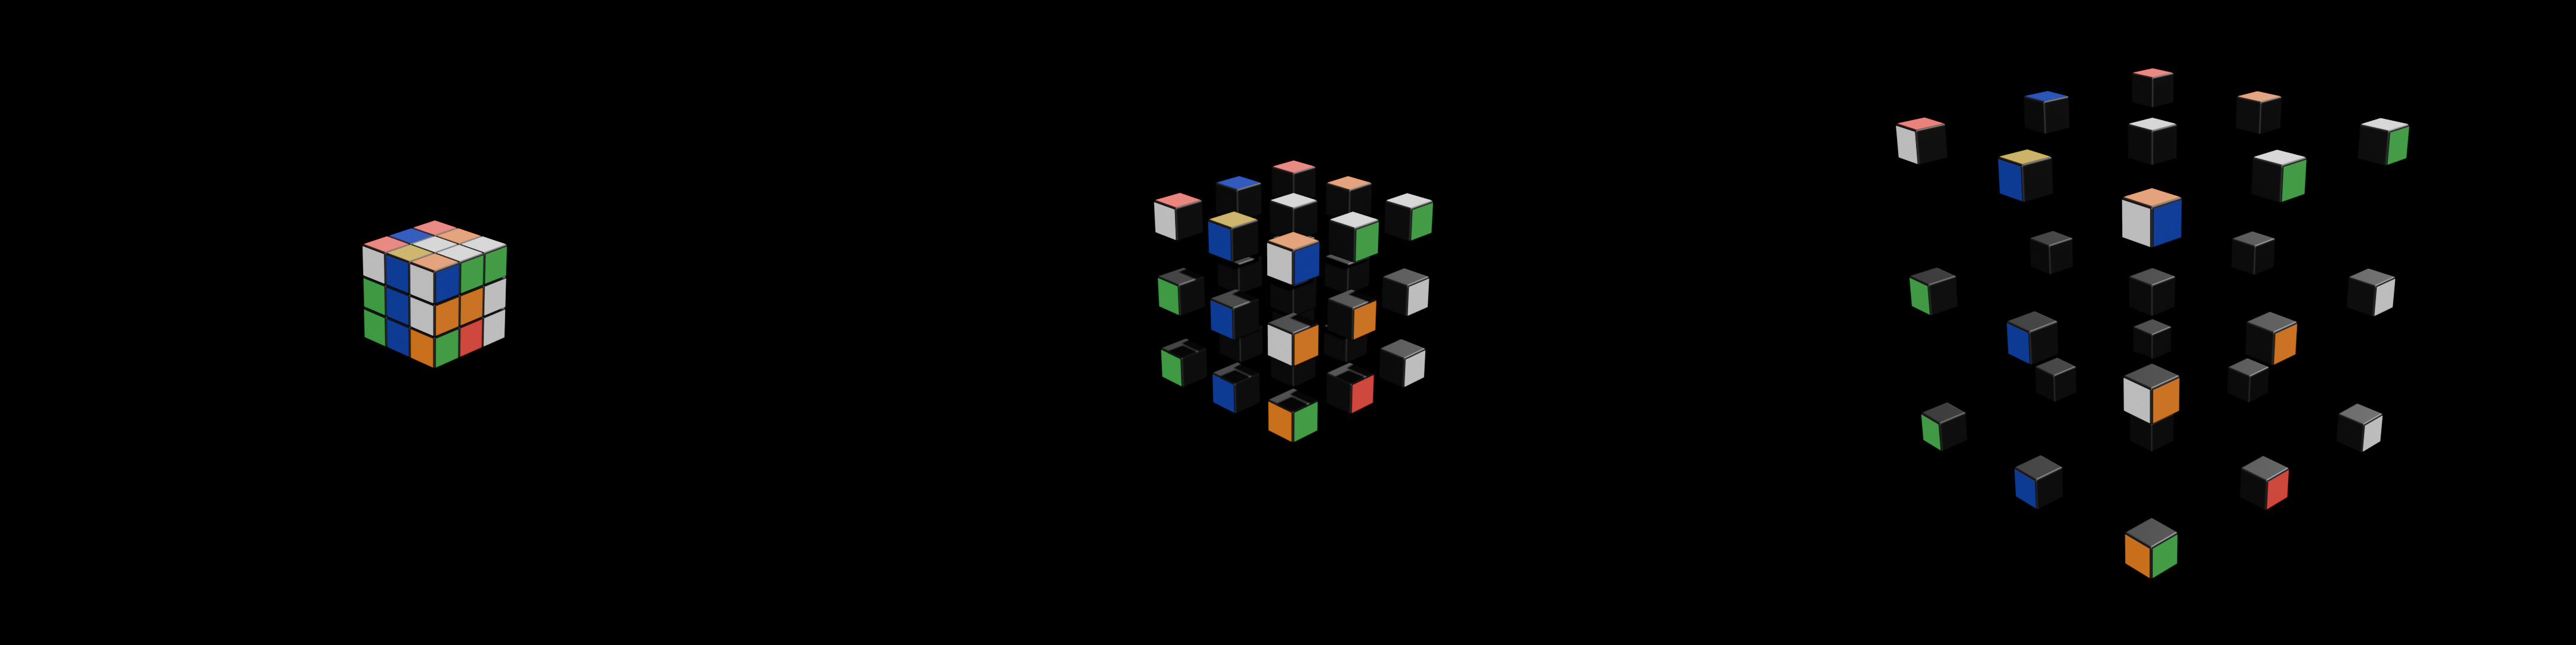
\includegraphics[width=1\textwidth]{images/RubiksExplosion.png}
    \caption{Beispiel einer Explosionsanimation anhand eines Rubiks Cube}
    \label{fig:rubiks-explosion}
\end{figure}

Die Anforderungen sollen dabei in Form von Text auf UI-Panels dargestellt werden, welche an den zugehörigen Bauteilen angebracht sind.

Da jedoch bei komplexeren Produkten mit sehr vielen Bauteilen, wie das zuvor genannte Beispiel des Autos, so würde eine gleichzeitige Animation aller Komponenten zu zu vielen Requirements führen, die gleichzeitig dargestellt werden sollten.
Daher ist es bei umfangreichen Produkten eventuell sinnvoll, die Darstellung der Bauteile in mehreren Schritten zu realisieren.
Dafür könnten Bauteile des Produkts, die aus mehreren anderen Bauteilen bestehen, als eigene Produkte mit ihrer eigenen Explosionsanimation betrachtet werden.
Zum Beispiel könnte in einer Komplettübersicht das gesamte Auto in wenigen Bauteilen dargestellt werden, indem beispielsweise ein Rad, das eigentlich aus Reifen, Felge, Radmuttern, Bremsscheibe etc. besteht, als ein einzelnes zusammengehöriges Objekt behandelt wird.
Will der Nutzer dann die Räder genauer betrachten, kann er in eine Detailansicht wechseln, in der nur ein Rad mit all seinen Bauteilen animiert wird.
So lässt sich durch eine Verschachtelung von immer detaillierteren Ansichten eine hohe Komplexität der Darstellung erreichen, ohne dass die Übersichtlichkeit durch zu viele Requirements gleichzeitig verloren geht.


Für diese Darstellung soll der Nutzer zunächst mithilfe eines Controllers einen Ort für die Darstellung im Raum auswählen.
Dieser Ort wird als Ursprungspunkt für die Darstellung der Bauteile verwendet.
Dann soll der Nutzer die Explosionsanimation des gerade angezeigten Modells per Knopfdruck aktivieren können.
Dabei wird dann die Animation abgespielt und den Bauteilen sollen ihre Requirement-Panels angehängt werden.

Auch bei Software-Requirements ist es denkbar, diese in ihre Komponenten zu zerlegen und zu diesen Komponenten zugehörige Anforderungen darzustellen.
Jedoch bietet die Darstellung in AR bzw. VR hierbei quasi keine Vorteile im Gegensatz zu einer 2D-Darstellung auf einem Bildschirm.
Bei Software-Anwendungen ist die einfache Darstellung auf einem Bildschirm näher an der tatsächlichen Laufumgebung der meisten Softwares weshalb das Konzept eher für physische Produkte sinnvoll ist.

Schon bei der Konzeption des Konzepts wird klar, dass einige der Implementierungsschritte, wie beispielsweise das Erstellen der Animation, zeitaufwendig sein können.
Daher soll bei diesem Interaktionskonzept die Realisierbarkeit solcher Darstellungen für physische Produkte untersucht werden.
Dabei muss aufgrund des erwarteten hohen Zeitaufwands für die Implementierung die Kosten-Nutzen-Relation kritisch betrachtet werden.
Um trotzdem noch sinnvoll für den tatsächlichen Einsatz zu sein, muss das Interaktionskonzept sonst einen großen Mehrwert bei der Vermittlung der Requirements bieten.

\newpage
\section{Wolken von Anforderungen}

Der Ansatz der explodierenden Bauteile ist aufgrund der Individualität der Implementierung des Interaktionskonzepts sehr zeitaufwendig und komplex einzusetzen.
Zudem ist dieser Ansatz nur für die Darstellung von Produkten, also physischen Systemen, geeignet.
Daher wird ein weiteres Interaktionskonzept entwickelt, welches sich theoretisch auch automatisiert generieren lassen soll und für alle Arten von Anforderungen geeignet ist.

Außerdem soll versucht werden, eine Übersicht über mehr Requirements gleichzeitig zu erlangen, als im ersten Interaktionskonzept, um eine visuelle Darstellung vieler Anforderungen gleichzeitig zu ermöglichen.

Die grundlegende Idee ist, Anforderungen in Wolken von Texten darzustellen, also als wolkenförmige Gruppierungen von UI-Elementen im Raum.
Die UI-Elemente sollen dabei Panele sein, auf denen der Text der Anforderungen sowie weiter Information zu den Anforderungen stehen sollen.
Diese Panele sollen dann in einer Wolkenartigen Anrichtung, ähnlich wie die Punktewolke in Abbildung , dargestellt werden.

\begin{figure}[H]
    \centering
    \includegraphics[width=0.6\textwidth]{images/PointCloud.jpg}
    \caption{Beispiel einer Punktewolke}
    \source{\autocite{PointCloud}}
    \label{fig:point-cloud}
  \end{figure}



Hierbei soll dann eine räumliche Gruppierung der Anforderungen nach verschiedenen Kriterien möglich sein.
Beispielsweise könnten Anforderungen, die zu einem bestimmten Feature gehören, in einer Wolke gruppiert werden, während Anforderungen, die zu einem anderen Feature gehören, in einer anderen Wolke gruppiert werden.
Durch die räumliche Anordnung der Wolken kann der Nutzer schnell erkennen, welche Anforderungen nach der aktuellen Filterung nah zuneinander liegen und welche nicht.

Dabei soll es auch möglich sein in Wolken hinein- und herauszuzoomen, um die Granularität der angezeigten Anforderungen zu erhöhen.
Beispielsweise könnten in großen Wolken initial nur Punkte als Repräsentationen von Requirements angezeigt werden, in welche man hereinzoomen kann um die Requirements zu lesen.
Daraufhin kann wieder herausgezoomt werden, um wieder eine Übersicht über mehr Requirements der Wolke zu erlangen.
Eine weitere Möglichkeit wäre es, auf den Anforderungspanels Filtermöglichkeiten für verschiedene Beziehungen der Anforderung darzustellen, um dann bei einer Auswahl in die neue Anforderungswolke zu wechseln.
Diese Interaktion und die räumliche Anordnung der Wolken sollen dem Nutzer helfen, auch bei einer großen Anzahl von Anforderungen einen Überblick zu behalten und schnell die gewünschten Anforderungen zu finden.

Bei diesem Konzept soll vor allem der Vorteil gegenüber einer 2D-Darstellung kritisch untersucht werden.
Denn die Darstellung der Anforderungen in Wolken ist prinzipiell auch in 2D möglich, auch mit der Interaktionsmöglichkeit des Hinein- und Herauszoomens.
Daher soll untersucht werden, ob die räumliche Anordnung der Anforderungen in AR tatsächlich einen Mehrwert gegenüber einer 2D-Darstellung bietet und ob die Interaktionen intuitiv und effizient sind.
Zudem soll ein Fokus darauf liegen, auch große Zahlen von Requirements gleichzeitig darzustellen.